 
 \subsection{Analytical versus numerical evaluation of the double derivative}
 
First we look at the difference between calculating the double derivative numerically and analytically. Table \ref{tab:compare_ana_num} shows how the CPU time is larger for the numerical derivation already at one particle in three dimensions. The ratio between the two rapidly increase when the number of particles increase. It is expected that the numerical derivation is slow because every particle is moved both back and forth in every dimension, to calculate the double derivative numerically. This is a major operation compared to calculation the squared sum of the position of every particle, which is how it is calculated analytically (see Appendix \ref{sec:implementation}).
 
\begin{table}[H]\caption{A comparison of the CPU time of calculating the double derivative analytically and numerically. Here N is the number of particles and these calculations were performed in three dimensions. The numbers in the table are an average of 10 runs.}\label{tab:compare_ana_num}
\center
\begin{tabular}{l|ll|l}
& CPU time [s]&\\
N & Analytical & Numerical & Ratio $\nicefrac{num}{ana}$\\ \hline
1 & 1.6319 & 2.7882 & 1.7085\\
2 & 2.3090 & 8.2743 & 3.5835\\
4 & 3.5503 & 14.5833 & 4.1076\\
6 & 4.7517 & 29.1024 & 6.1246\\
8 & 6.0642 & 48.4739 & 7.9934\\
10 & 7.6771 & 67.4531 & 8.7863\\
\end{tabular}
\end{table}

\subsection{No interaction - brute force sampling}

\subsubsection{Comparison with exact values}

Figure \ref{fig:exact_comparison_1D} shows the energies of the Bose gas. These calculations were performed with brute force sampling and the particles are not interacting with each other. The exact energy for $N$ number of particles in $d$ dimensions is given by

\begin{equation}\label{eq:exact_energy_expression}
\left< E \right> =\left( \frac{1}{2}\alpha + \frac{1}{8 \alpha}\right)Nd
\end{equation}

which was found from the one particle in one dimension case in Ref. \cite{GriffithsDavidJ1995Itqm}. Equation \ref{eq:exact_energy_expression} is in natural units where $m = 1$, $\hbar = 1$ and $\omega = 1$. The parameter that gives the minimum of the exact energy is easily found from the derivative of Eq. \ref{eq:exact_energy_expression} with respect to $\alpha$
$$ \frac{d \left<E\right>}{d \alpha}  = \left(\frac{1}{2} - \frac{1}{8\alpha^2}\right)Nd = 0 \implies \alpha = \frac{1}{2}. $$
The energy when $\alpha = 0.5$ is then
$$ \left< E(\alpha = 0.5)\right> = \left(\frac{1}{4} + \frac{2}{8}\right)Nd = \frac{1}{2}Nd $$
We see that this is the case in Fig. \ref{fig:exact_comparison_1D}, where all the energies follow the exact curve since the energy is plotted in energy per particle and all calculations are done in one dimension. We observe some variations from the exact values, but the calculation were done with only $2^{19} \approx 5.2\cdot10^{5}$ MC cycles and might have gotten closer to the exact with more cycles.

\begin{figure}[H]
\center
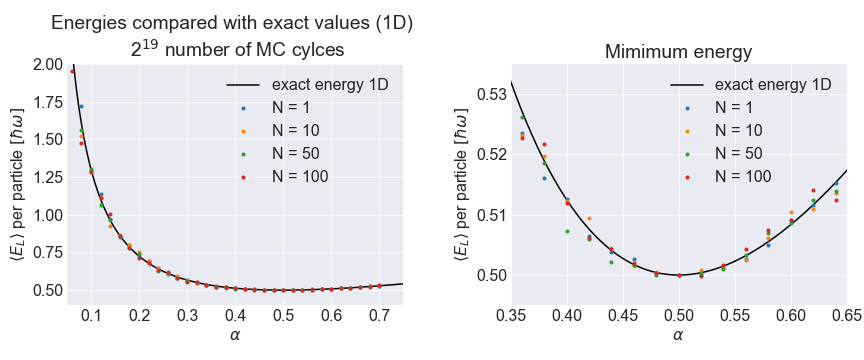
\includegraphics[width=\linewidth]{../Results/comparing_with_exact_1D}\caption{Energy of the boson gas for a range of different parameters $\alpha$. Here $N$ is the number of particles. And the exact energy is calculated using Eq. \ref{eq:exact_energy_expression}. Left: The exact energy for one particle in one dimension including the calculated energies per particle, so they can be easily compared. Right: A closer look at the minimum point of the curve.}\label{fig:exact_comparison_1D}
\end{figure}

%\begin{table}[H]\caption{Exact expectation values for the systems relevant in this project. Here $d$ is the number of dimensions and $N$ is the number of particles. The energies are of units $\hbar \omega_{ho}$.}\label{tab:exact_values}
%\center
%\begin{tabular}{rrr|rrr|rrr}
%$d$ & $N$ & $\left< E_L \right>$ &$d$ & $N$ & $\left< E_L \right>$&$d$ & $N$ & $\left< E_L \right>$\\ \hline
%&1 & 0.5 &&1 & 1.0 &&1 & 1.5\\
%&10 & 5.0&&10 & 10.0 &&10 & 15.0\\
%1& 50 & 25.0 &2& 50 & 50.0& 3& 50 & 75.0 \\
%&100 & 50.0 &&100 & 100.0 &&100 & 150.0 \\
%&500 & 250.0 &&500 & 500.0& &500 & 750.0 \\ 
%\end{tabular}
%\end{table}

 \subsubsection{Brute force sampling}
 
Table \ref{tab:brute_force_N_1_MC_20} shows the calculated energies for one particle in three dimensions. We observe that the difference between the exact energies and the calculated energies are sometimes smaller than the standard deviation calculated from the blocking resampling method which should give us an estimate of the error. This is suprising, but we also observe that the normal standard deviation, $\sigma$, which should underestimate the error is larger than the standard deviation from the blocking resampling method, $\sigma_B$. In Appendix \ref{app:alpha_lists_brute_force} we have the results for the same calculations for $2^{24}$ MC cycles, but the same trend is observed there.

\begin{table}[H]\caption{The calculated energies, $\left<E_L\right>$, for one particle in three dimensions compared with the exact energy, $E_{ex}$. Both energies are of units $\hbar\omega_{oh}$. These calculations were performed with $2^{20}$ number of MC cycles. The normal standard deviation $\sigma$, and the variance from the blocking resampling method, $\sigma_B$ are also included. }\label{tab:brute_force_N_1_MC_20}
\center
\begin{tabular}{cccccc}
$\alpha$ & $\left< E_L \right>$ & $E_{ex}$ & |$\left< E_L \right>-E_{ex}$|  & $\sigma_B$ & $\sigma$\\ \hline
0.35 & 1.59503 & 1.59643 & 0.00139 & 0.00536 & 0.44488\\
0.40 & 1.53597 & 1.53750 & 0.00153 & 0.00304 & 0.27225\\
0.45 & 1.50667 & 1.50833 & 0.00166 & 0.00141 & 0.12795\\
0.50 & 1.50000 & 1.50000 &                &                &                 \\
0.55 & 1.50519 & 1.50682 & 0.00163 & 0.00119 & 0.11732\\
0.60 & 1.52287 & 1.52500 & 0.00213 & 0.00238 & 0.22638\\
0.65 & 1.54415 & 1.55192 & 0.00777 & 0.00328 & 0.32873\\
\end{tabular}
\end{table} 

Table \ref{tab:brute_force_N_10_MC_20} shows the  calculated energies for ten particles in three dimensions. Here we observe a similar behavoir as the one particle system. The normal standard deviation, is greatly overestimating the error and it shows a strange behaviour. We would expect the normal standard deviation to give a much smaller standard deviation than the one from the blocking resampling method because the latter includes an estimate of the correlation in our data set. Figure \ref{fig:histogram} shows the distribution of the local energies for the system in Tab. \ref{tab:brute_force_N_10_MC_20} for $\alpha = 0.45$. We observe from the width of the distribution that a standard deviation of $0.4$, which is the normal standard deviation, is reasonable. The tail at the positive side of the mean could also contribute to increase the normal standard deviation. Another explanation of the large standard deviation could be an outlier, e.g. a very large number, therefore I checked the values in Excel by sorting them from the largest to the smallest. Hence extracting the minimum and maximum, but I found a minimum at 13.8677 and a maximum at 17.6977, so there are no outliers. 


\begin{table}[H]\caption{The calculated energies, $\left<E_L\right>$, for ten particles in three dimensions compared with the exact energy, $E_{ex}$. Both energies are of units $\hbar\omega_{oh}$. These calculations were performed with $2^{20}$ number of MC cycles. The normal standard deviation, $\sigma$, and the standard deviation from the blocking resampling method, $\sigma_B$ are also included.}\label{tab:brute_force_N_10_MC_20}
\center
\begin{tabular}{cccccc}
$\alpha$ & $\left< E_L \right>$ & $E_{ex}$ & |$\left< E_L \right>-E_{ex}$|  & $\sigma_B$ & $\sigma$\\ \hline
0.35 & 15.97857 & 15.96429 & 0.01429 & 0.05287 & 1.42240\\
0.40 & 15.43743 & 15.37500 & 0.06243 & 0.03071 & 0.87692\\
0.45 & 15.07640 & 15.08333 & 0.00693 & 0.01373 & 0.40780\\
0.50 & 15.00000 & 15.00000 &                &                &                \\
0.55 & 15.07949 & 15.06818 & 0.01131 & 0.01095 & 0.36979\\
0.60 & 15.22724 & 15.25000 & 0.02276 & 0.02066 & 0.71239\\
0.65 & 15.54577 & 15.51923 & 0.02653 & 0.02772 & 1.00763\\
\end{tabular}
\end{table} 

\begin{figure}[H]
\center
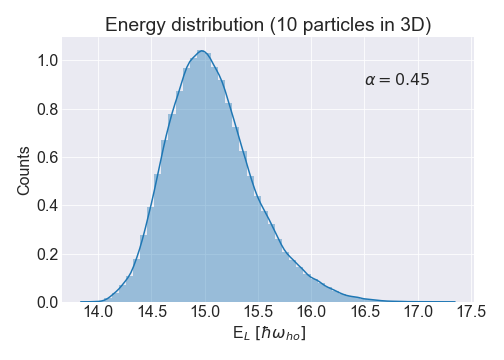
\includegraphics[width=0.5\linewidth]{../Results/histogram_10p_3d_alpha_45}\caption{A histogram of the local energy distribution for the calculation where $\alpha = 0.45$ in Tab. \ref{tab:brute_force_N_10_MC_20}.}\label{fig:histogram}
\end{figure}

The resulting energies and standard deviations for calculations of the system with higher number of particles (50 particles, 100 particles and 500 particles) can be found in Appendix \ref{app:alpha_lists_brute_force}. Those calculations show a similar behaviour, the only difference being that they have higher energies, and were therefore not included here. 

\subsection{Including importance sampling}

Figure \ref{fig:compare_importance_steps} shows that with brute force sampling there seems to be a trade-off between the acceptance and the accuracy of the result. The right plot shows that larger steps, to a certain point, will give a better accuracy, but, as can be observed in plot to the left, the acceptance decreases with larger step lengths, $dl$. We also see that for smaller step sizes, the brute force sampling's accuracy is very poor, at least for $2^{20}$ number of MC cycles. From the comparison of the two plots a  step length at $dl = 0.5 = 5\cdot10^{-1}$ seems to give the best trade-off when using brute force sampling with $2^{20}$ number of MC cycles.

With importance sampling, on the other hand, both acceptance and accuracy increases with smaller time steps ($\Delta t$). A time step at $\Delta t = 0.005 = 5\cdot10^{-3}$ seems to be a good choice with $2^{20}$ number of MC cycles according to Fig. \ref{fig:compare_importance_steps}. 

\begin{figure}[H]
\center
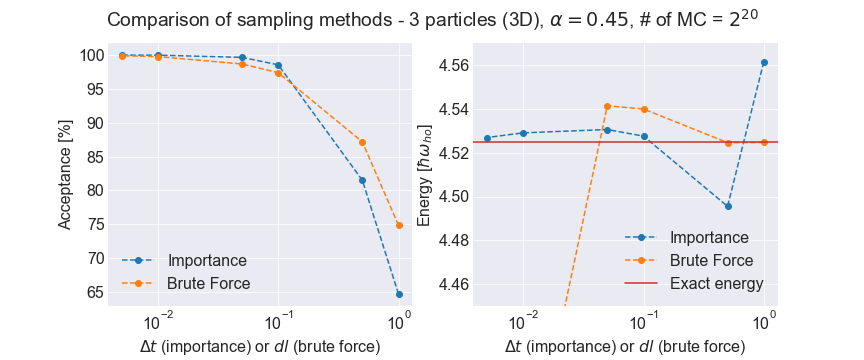
\includegraphics[width=\linewidth]{../Results/comparison_steps_importance}\caption{A comparison between brute force sampling and importance sampling. Left: The acceptance percent of suggested moved as a function of step length ($dl$) or time step ($\Delta t$). Right: The expectation value of the energy after $2^{20}$ steps and $\alpha = 0.45$ compared with the exact energy $\alpha = 0.45$. }\label{fig:compare_importance_steps}
\end{figure}

Figure \ref{fig:compare_importance_MC} was made using the step sizes extracted from Fig. \ref{fig:compare_importance_steps}. The figure shows that both sampling methods give accurate values (within $\pm$ 0.004 of the exact value) for number of MC cycles above $2^{20}$, at least for three particles in three dimensions.

\begin{figure}[H]
\center
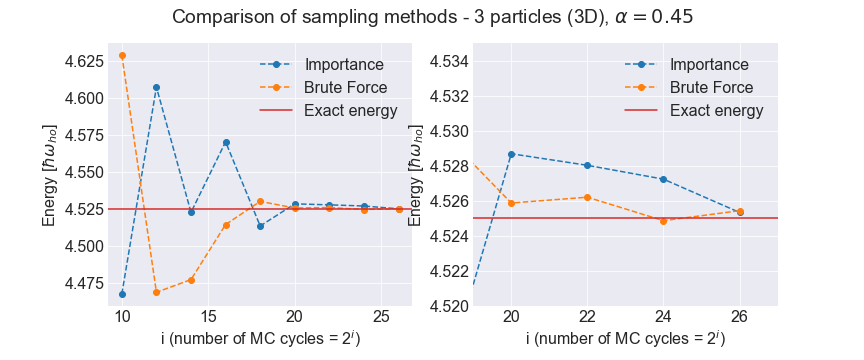
\includegraphics[width=\linewidth]{../Results/comparison_MC_importance}\caption{A comparison of the behaviour of the different sampling methods with regards to number of MC cycles.}\label{fig:compare_importance_MC}
\end{figure}

Table \ref{tab:importance_N_1} and \ref{tab:importance_N_10} show the resulting energies and standard deviations from calculations with importance sampling for one and ten particles in three dimensions respectively. The numbers are very similar to the calculated values from the brute force sampling method, but this is expected from the results in Fig. \ref{fig:compare_importance_steps} and \ref{fig:compare_importance_MC} which show that the expectation energies from the two methods are similar with number of MC cycles above $2^{20}$ and an appropriate $dl$ or $\Delta t$. 

\begin{table}[H]\caption{The calculated energies, $\left<E_L\right>$, for one particle in three dimensions compared with the exact energy, $E_{ex}$. Both energies are of units $\hbar\omega_{oh}$. These calculations were performed with $2^{20}$ number of MC cycles. The normal standard deviation $\sigma$, and the variance from the blocking resampling method, $\sigma_B$ are also included. }\label{tab:importance_N_1}
\center
\begin{tabular}{cccccc}
$\alpha$ & $\left< E_L \right>$ & $E_{ex}$ & |$\left< E_L \right>-E_{ex}$|  & $\sigma_B$ & $\sigma$\\ \hline
0.35 & 1.59139 & 1.59643 & 0.00504 & 0.00965 & 0.43954\\
0.40 & 1.53229 & 1.53750 & 0.00521 & 0.00550 & 0.27462\\
0.45 & 1.50692 & 1.50833 & 0.00141 & 0.00243 & 0.12940\\
0.50 & 1.50000 & 1.50000 &                &                &                 \\
0.55 & 1.50696 & 1.50682 & 0.00014 & 0.00201 & 0.11744\\
0.60 & 1.52597 & 1.52500 & 0.00097 & 0.00343 & 0.22232\\
0.65 & 1.55742 & 1.55192 & 0.00549 & 0.00509 & 0.32402\\
\end{tabular}
\end{table} 

\begin{table}[H]\caption{The calculated energies, $\left<E_L\right>$, for ten particles in three dimensions compared with the exact energy, $E_{ex}$. Both energies are of units $\hbar\omega_{oh}$. These calculations were performed with $2^{20}$ number of MC cycles. The normal standard deviation, $\sigma$, and the standard deviation from the blocking resampling method, $\sigma_B$ are also included.}\label{tab:importance_N_10}
\center
\begin{tabular}{cccccc}
$\alpha$ & $\left< E_L \right>$ & $E_{ex}$ & |$\left< E_L \right>-E_{ex}$|  & $\sigma_B$ & $\sigma$\\ \hline
0.35 & 15.98097 & 15.96429 & 0.01668 & 0.09399 & 1.47776\\
0.40 & 15.33029 & 15.37500 & 0.04471 & 0.04686 & 0.85013\\
0.45 & 15.07401 & 15.08333 & 0.00932 & 0.02182 & 0.38900\\
0.50 & 15.00000 & 15.00000 &                &                &                \\
0.55 & 15.07112 & 15.06818 & 0.00294 & 0.01612 & 0.36242\\
0.60 & 15.19266 & 15.25000 & 0.05734 & 0.03098 & 0.70746\\
0.65 & 15.54807 & 15.51923 & 0.02884 & 0.04239 & 0.98210\\
\end{tabular}
\end{table} 

\subsection{Including optimization with simple  gradient descent methods}

We will now look at optimization and specifically the simple gradient descent methods described in section \ref{sec:gradient} and \ref{sec:gradient2}. How the important factor $\frac{\partial \left< E_L\right>}{\partial \alpha}$ is found is described in Appendix \ref{app:alpha_derivative}.

Figure \ref{fig:gradient_descent_starts} shows how the efficiency of the simple gradient descent method is dependant on the first guess, the start value of $\alpha$. We observe that, naturally, the algorithm is faster when the guess is closer to the exact parameter ($\alpha = 0.5$). 

\begin{figure}[H]
\center
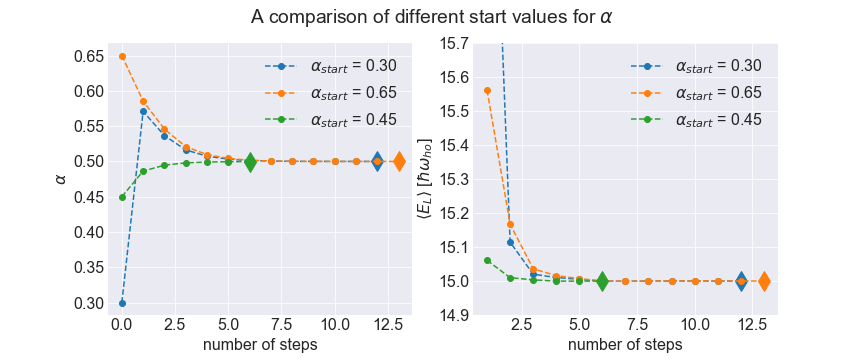
\includegraphics[width=\linewidth]{../Results/gradient_descent_starts}\caption{A comparison of different start values for the parameter $\alpha$. The algorithm stops when the energy difference is less then $1\cdot10^{-5}$ from one step to the next. The diamond shape marker is added to emphasis at what step this criteria is fulfilled. These calcualtions are made for ten particles in three dimensions. Left: The development of $\alpha$. Right: the development of the expectation value.}\label{fig:gradient_descent_starts}
\end{figure}

Figure \ref{fig:gradient_descent_rates} shows that the minimization rate, $\gamma$, should not be chosen to be too small, then the algorithm moves very slowly toward the minimum as observed for $\gamma= 0.01$. On the other hand, if the rate is too big it also moves slowly toward the $\alpha$ that gives the minimum, but oscillating between values larger and smaller than the $\alpha$ that gives the minimum energy. From the figure we observe that $\gamma = 0.2$ is the most effective minimization rate.

\begin{figure}[H]
\center
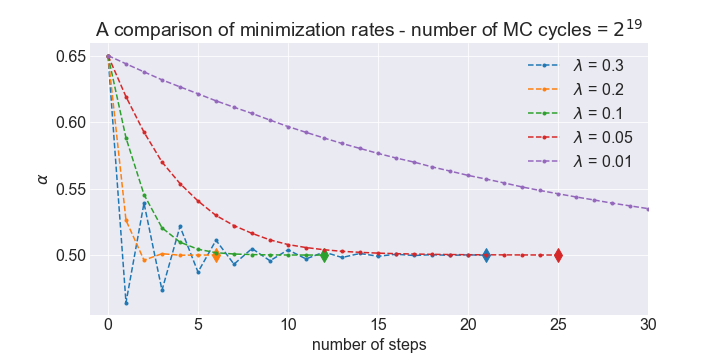
\includegraphics[width=0.8\linewidth]{../Results/gradient_minimization_rate}\caption{A comparison of different minimization rates using the simple gradient descent method from section \ref{sec:gradient}. Here $\lambda$ is the minimization rate. The diamond markers are used to show at which step the difference between the last two energies were less than $1\cdot 10^{-5}$.} \label{fig:gradient_descent_rates}
\end{figure}

Figure \ref{fig:gradient_descent_lambda} shows how the simple gradient descent method can be made more efficient by including the gradient calculated for the previous step. Similarly to the evaluation of $\gamma$, a $\lambda$ that is not too small ( too small $\lambda$ will result in the same result as for the simple gradient descent method) and not too large has to be found. Here we observe that $\lambda = 0.02$ is the best choice when $\gamma = 0.1$. Even though this more complex gradient method can make the simple gradient method more effective the difference is not crucial for this project and the simple gradient descent method is good enough.

\begin{figure}[H]
\center
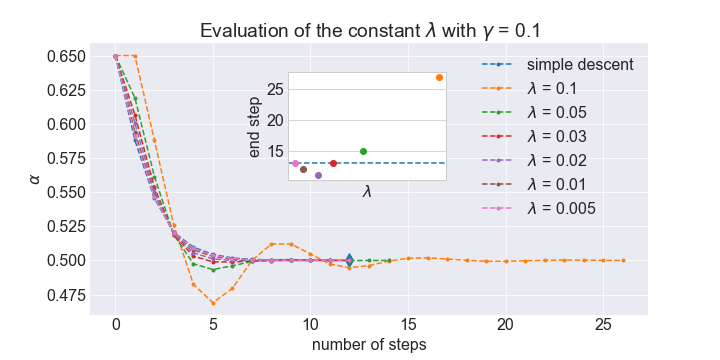
\includegraphics[width=0.8\linewidth]{../Results/comparing_gradient_descents.png}\caption{A comparison of the two gradient descent methods described in section \ref{sec:gradient} and \ref{sec:gradient2}. The algorithm stops when the energy difference is less then $10^{-5}$ from one step to the next. Here $\lambda$ is the weight of the previous gradient's influence on the next pick of $\alpha$. The inset plot shows how many steps is needed to reach this criteria the different $\lambda$s. The dotted blue line shows the number of steps needed for the simple gradient descent method.}\label{fig:gradient_descent_lambda}
\end{figure}



\subsection{Including interaction and an elliptical trap}

Here we have added an interaction potential in the Hamiltonian and hence included an interaction term in the wavefunction. This is all described in the theory part of this report and how it is implemented in the code to calculate the local energy and the drift force is described in Appendix \ref{sec:implementation}. The change of the Hamiltonian is described in detail in Appendix \ref{app:new_Hamiltonian}.

Table \ref{tab:interaction_N_10} and \ref{tab:interaction_N_50} show the resulting expectation values for a range of $\alpha$s for a system with ten and fifty particles in three dimensions respectively. The tables show that the minimum energy is still found with $\alpha = 0.5$ for both systems, but this is only a range of selected $\alpha$s. We therefore have to employ optimization with the gradient descent method to find the true $\alpha$ that gives the minimum. We also observe that the energy is higher than the exact energy for the case with not interacting particles. The higher energy seems reasonable since the interaction is repulsive, so the particles prefer it less, i.e. to be trapped in the magnetic trap with the other particles.

\begin{table}[H]\caption{The calculated energies, $\left<E_L\right>$, for ten particles in three dimensions compared with the exact energy for the non-interacting case, $E_{ex}$. Both energies are of units $\hbar\omega_{oh}$. These calculations were performed with $2^{20}$ number of MC cycles. The normal standard deviation, $\sigma$, and the standard deviation from the blocking resampling method, $\sigma_B$ are also included.}\label{tab:interaction_N_10}
\center
\begin{tabular}{cccccc}
$\alpha$ & $\left< E_L \right>$ & $E_{ex}$(no int.) & |$\left< E_L \right>-E_{ex}$|  & $\sigma_B$ & $\sigma$\\ \hline
0.35 & 16.16895 & 15.96429 & 0.20466 & 0.04723 & 1.39931\\
0.40 & 15.57277 & 15.37500 & 0.19777 & 0.02440 & 0.82444\\
0.45 & 15.33414 & 15.08333 & 0.25080 & 0.01153 & 0.37842\\
0.50 & 15.25790 & 15.00000 & 0.25790 & 0.00120 & 0.07902\\
0.55 & 15.35359 & 15.06818 & 0.28541 & 0.01228 & 0.41498\\
0.60 & 15.58890 & 15.25000 & 0.33890 & 0.01847 & 0.74266\\
0.65 & 15.84713 & 15.51923 & 0.32789 & 0.02895 & 1.09169\\
\end{tabular}
\end{table} 

\begin{table}[H]\caption{The calculated energies, $\left<E_L\right>$, for fifty particles in three dimensions compared with the exact energy for the non-interacting case, $E_{ex}$. Both energies are of units $\hbar\omega_{oh}$. These calculations were performed with $2^{20}$ number of MC cycles. The normal standard deviation, $\sigma$, and the standard deviation from the blocking resampling method, $\sigma_B$ are also included.}\label{tab:interaction_N_50}
\center
\begin{tabular}{cccccc}
$\alpha$ & $\left< E_L \right>$ & $E_{ex}$(no int.) & |$\left< E_L \right>-E_{ex}$|  & $\sigma_B$ & $\sigma$\\ \hline
0.35 & 85.11556 & 79.82143 & 5.29413 & 0.19303 & 3.00642\\
0.40 & 82.50113 & 76.87500 & 5.62613 & 0.10011 & 1.71066\\
0.45 & 81.59128 & 75.41667 & 6.17461 & 0.04225 & 0.72452\\
0.50 & 81.54031 & 75.00000 & 6.54031 & 0.02800 & 0.45609\\
0.55 & 82.44027 & 75.34091 & 7.09936 & 0.07706 & 1.28038\\
0.60 & 83.93794 & 76.25000 & 7.68794 & 0.11619 & 2.04841\\
0.65 & 85.52708 & 77.59615 & 7.93093 & 0.17015 & 2.83331\\
\end{tabular}
\end{table} 

Figure \ref{fig:interaction_gradient_descent_N_10} shows the result of the simple gradient descent method for ten particles. Here we used the $\alpha$ that gave the minimum expectation value for the not interacting system as the starting point, i.e. $\alpha = 0.5$. From the plots of the derivative of the expectation energy we observe that the gradient descent method is oscillating around the minimum. Therefore a mean value of the $\alpha$s from step 20 and to the end were extracted and found to be $\bar{\alpha}_{15\rightarrow} = 0.495934$. The same procedure was performed to find the optimal alpha for other systems with different number of particles and the result is in Tab. \ref{tab:interaction_vs_not}. To compare fairly with the not interacting case the same procedure was performed for those cases. Here we pretend not to know the exact $\alpha$ that gives the minimum energy and start with a guess for $\alpha$ that is $\alpha = 0.51$. The result of this is showed together with the interacting case in Tab. \ref{tab:interaction_vs_not}. 

\begin{figure}[H]
\center
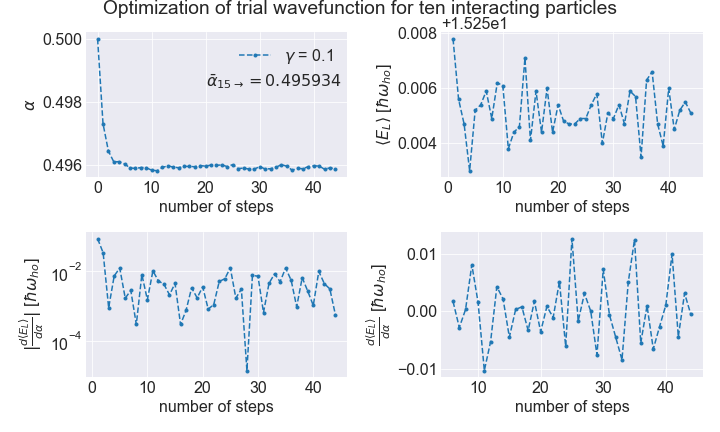
\includegraphics[width=\linewidth]{../Results/gradient_descent_interaction_10p}\caption{Upper left: The development of the parameter $\alpha$ during the simple gradient descent method with $\gamma = 0.1$. In the plot the mean value, $\bar{\alpha}$, of the $\alpha$s from step 15 and to the end is showed. Upper right: The expectation energy for the system with ten particles in 3D. Lower left: The absolute value of the derivative of alpha used in the simple gradient descent method. Lower right: The derivative of alpha used in the simple gradient descent method. }\label{fig:interaction_gradient_descent_N_10}
\end{figure}

From Tab. \ref{tab:interaction_vs_not} we see that $\alpha$ seems to get smaller for larger amounts of particels when we have included interaction. And, as we have seen before, the energy is larger than the ground state when there is no interaction.

\begin{table}[H]\caption{$\left<E_L\right>$ for different amount of particles in three dimensions calculated at the $\alpha$ found from the gradient descent method. Energies are of units $\hbar\omega_{oh}$. These calculations were performed with $2^{20}$ number of MC cycles. The normal standard deviation, $\sigma$, and the standard deviation from the blocking resampling method, $\sigma_B$ are also included.}\label{tab:interaction_vs_not}
\center
\begin{tabular}{c|c}
Interacting particles and elliptical trap &No interaction and spherical trap\\
\begin{tabular}{ccccc}
N &$\alpha$ & $\left< E_L \right>$ & $\sigma_B$ & $\sigma$\\ \hline
10 &0.495934 & 15.25500 & 0.00054 & 0.04169\\
50 &0.483195 & 81.46368 & 0.00987 & 0.31798\\ 
\end{tabular}&
\begin{tabular}{ccccc}
N &$\alpha$ & $\left< E_L \right>$ & $\sigma_B$ & $\sigma$\\ \hline
10 & 0.500015 & 14.99999 & 0.00000 & 0.00012\\
50 & 0.500073 & 74.99985 & 0.00004 & 0.00131\\
\end{tabular}
\end{tabular}
\end{table} 

\subsection{One-body densities}

The one-body density was evaluated by dividing the x-, y- and z-axis into 800 bins between -5 and 5. Then, every time the energy was sampled the positions of the particles were checked. The positions where checked like as such; the x-coordinate of the particle was checked and if the x-value fell within one of the bins on the x-axis that bin got a count. This was done for all dimensions and all particles. In the end all MC cycles, the counts in the bins where normalized by dividing with the number of MC cycles and the number of particles. Furthermore, when plotting the one-body density, the normalized counts in every bin was made into a length like this

$$\text{counts in bin $i$} =  \sqrt{ (\text{x$_i$-counts})^2 + (\text{y$_i$-counts})^2 + (\text{z$_i$-counts})^2}.$$

At last, the counts in the bins representing the negative values where added to the bins representing the same positive values.

Figure \ref{fig:one_body_density_N_50} shows the one-body density of the system with fifty particles in the elliptical potential. We oberve a small difference between the case with out without the Jastrow factor. The trap size is probably a little  big compared to the amount of particles for us to be able to observe a large difference in the density. The difference we expect is that the case with interaction is spread out compared to the other case. This is because we have a repulsive interaction between the particles. A spreading out is also what we see in the figure.

\begin{figure}
\center
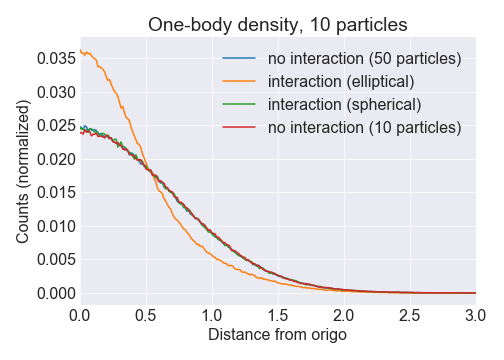
\includegraphics[width=0.7\linewidth]{../Results/one_body_density_10p}\caption{One-body denisty of a system of ten particles with and without the Jastrow factor.}\label{fig:one_body_density_N_50}
\end{figure}

\section{Concluding remarks}

In this project we found the ground state energy using the VMC method and we also explored different ways of making the code more compex and effective. We have implemented importance sampling and optimizing methods. To make the model more realistic, we implemented interaction and saw that this changed both the trial wavefunction and the energy in the ground state. 

There are some aspects of this project that were not ideal. For example the standard deviation calculated directly from the sampled local energies were large compared to what is expected. I tried to investigate it a little bit and specifically check if it really was high or if something made it look larger than is was i.e. and outlier. 

Another thing is that I only calcualted the energies and other things for maximum fifty particles in three dimensions. This was because the code was too slow to do any more. I tried to use optimizing flags etc, but they did not make the calcualtions any faster.I will definitly have to parallelize for the next project and maybe also use the supercomputer I have access to. I also had some issues with combining importance sampling and interaction. I could not find out what was wrong, so I decided to use brute force sampling for the interacting cases.
I also notices that when I found the equilibrium and number of MC cycles, I did this for only three particles in 3D and assumed that this would apply for more particles as well. This was probably not a great assumption, especially for the equilibration, since a higher number of particles probably acquire more steps to get to a steady state since we only move one particle at the time. At last I want to comment that when I looked at different minimization rates I chose the change in energy smaller than $10^{-5}$ as a criteria to stop the gradient descent. Afterward I thought it might be a bad idea because it does not nescarily mean that it is at a steady state and it could be random. Therefore I used a  different method to find $\alpha$ later.


% \begin{equation}
% E_L = -\frac{\hbar^2}{2m} \sum_k^N \left( \frac{\partial^2}{\partial x_k^2} \phi(x_k,y_k,z_k)  + \frac{\partial^2}{\partial y_k^2} \phi(x_k,y_k,z_k) + \frac{\partial^2}{\partial z_k^2} \phi(x_k,y_k,z_k) \right) + \frac{1}{2}m \omega^2 \sum_k^N \left( x_k^2 + y_k^2 +z_k^2 \right)
% \end{equation}